S Bre{ß} and others developed CoGaDB architecture to be highly efficient and modularized as shown in top-down approach in Figure \ref{fig:cogadbarch}. As most DBMSs, CoGaDB provides SQL frontend interface which can be used to write SQL language queries and launch it to get results from database. The SQL interface converts the provided language query into abstract syntax tree which is then pushed to logical optimizer module after being converted into a logical plan. Then, CoGaDB's logical optimizer applies pre-defined optimization policies on the logical plan such as pushing down selections, cross products resolution and reviewing join conditions. After this, the more efficient logical query plan is provided to HyPE for processing.
\begin{figure}
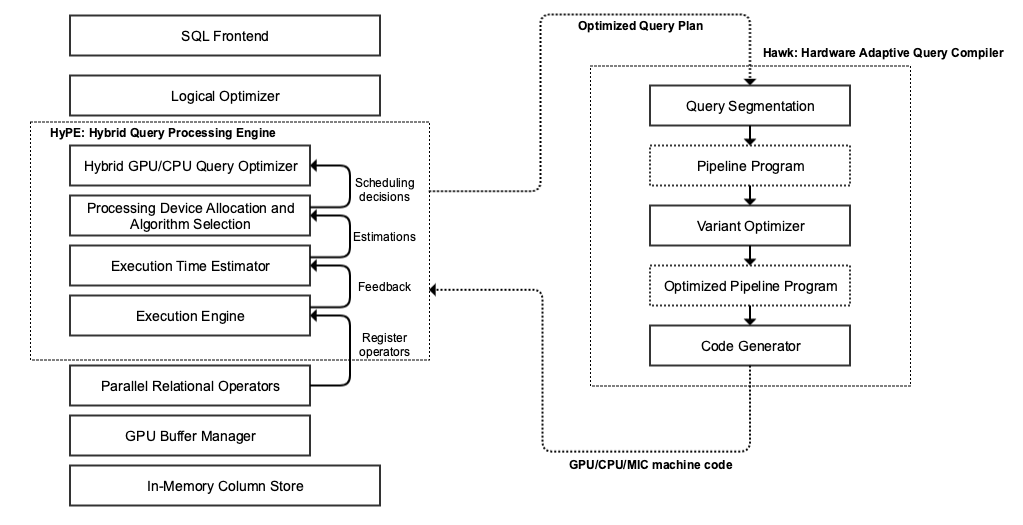
\includegraphics[width=\textwidth]{cogadb/cogadb_hawk_architecture}
\caption{The architecture of CoGaDB, adapted from \cite{cogadb_hawk} and \cite{cogadb_manual}}
\label{fig:cogadbarch}
\end{figure}
\newline
Hybrid Query Processing Engine(HyPE)\cite{cogadb_hype} is used as the physical optimizer for CoGaDB. HyPE has three main components: Hybrid GPU/CPU Query Optimizer, a processing device allocator and algorithm selector, and an execution time estimator module, which predicts the execution time on different possible processing device such as CPU, GPU or MIC. The hybrid query optimizer creates an optimized physical query plan from logical query plan using the time estimator and algorithm selector components\cite{cogadb_manual}. Using the analysis of these components, HyPE selects the most efficient processing device for the execution of the query and pass the query plan to Hawk for its most optimized machine code generation with respect to the selected processing device.
\newline
Hardware Adaptive Query Compiler(Hawk) uses the pipeline approach to transform the query plan into the required machine code variant. It performs query compilation, which compiles the query execution plans just-in-time into machine code of the target processor\cite{cogadb_hawk}. Hawk's code compilation provides a strong backbone to the execution engine of the HyPE and making CoGaDB highly hardware-oblivious.
\newline
GPU buffer manager is used to manage data transmission. It handles copying data to GPU for processing. It is also responsible for caching input columns to GPU, which is highly helpful in improving query performance in the case of similar query executions.
\newline
The entire query processor of CoGaDB is build upon in-memory, column-oriented storage. In case of memory crunch issues, virtual memory of the system is used, which is managed by database buffer system. Due to its in-memory data locality nature, CoGaDB can easily transfer data from CPU to GPU for processing and parallel executions, leading to high-throughput and extreme performance improvements. 